
\begin{figure*}
  \begin{center}
    \subfloat[Part A][\label{fig:delA}Both Process $a$ and
      Process $c$ initiate then remove a partition.
      $w_{ab} = 1.5$; $w_{bc} = w_{cd} = w_{bd} = 1$.]{
\begin{tikzpicture}[scale=\SCALE]

  \draw[opacity=0](-2.45*\X, 0) -- (2.45*\X, 0); %% more space for caption
  

  
  \draw (-\X + 5pt, 0) --
  node[above=-0.3em,font=\tiny]{$\DEL_{a} \RIGHT$}
  (0 - 5pt, 0); %% b - a 

  \draw (0 +5pt, 0) --
  (\X -5pt, 0); %% b - c

  \draw [<-] (0, 0 - 5pt) --
  (0, \Y + 5pt);  %% b - d
  
  \draw [<-] (\X + 3pt, 0 - 5pt) --
  (0 + 5pt, \Y - 3pt); %% c - d


  
  \draw[fill=white] (-\X, 0) node{$\bm{a}$} +(-5pt, -5pt) rectangle +(5pt, 5pt);  
  \draw[fill=white] (0, 0) node[color=\PD]{$\bm{b}$} +(-5pt, -5pt) rectangle +(5pt, 5pt);
  \draw[fill=white] (\X, 0) node[color=\PD]{$\bm{c}$} +(-5pt, -5pt) rectangle +(5pt, 5pt);
  \draw[fill=white] (0, \Y) node[color=\PD]{$\bm{d}$} +(-5pt, -5pt) rectangle +(5pt, 5pt);
  
  \draw (-\X, 5pt) node[above, font=\small]{$\DEL_a$};
  \draw (0, 5pt) node[above, font=\small, color=\PD]{$\ADD_d^1$};
  \draw (\X, 5pt) node[above, font=\small, color=\PD]{$\ADD_d^2$};
  \draw (-5pt, \Y) node[left, font=\small, color=\PD]{$\ADD_d^0$};


\end{tikzpicture}
}
    \hspace{5pt}
    \subfloat[Part B][\label{fig:delB}Process $b$ and Process $d$ receive and deliver
      messages based on their weights. $a$'s partition propagates to all processes.]
             {
\begin{tikzpicture}[scale=0.87]

  \thickmuskip=0mu
  \medmuskip=0mu
  \thinmuskip=0mu
  
  \newcommand\X{50pt}
  \newcommand\Y{-50pt}

  \newcommand\ADD{\alpha}
  \newcommand\DEL{\delta}



  \draw (-\X + 5pt, 0) --
  node[above=-0.3em,font=\tiny]{$\DEL_{a} \rightarrow$}
  node[below=-0.3em,font=\tiny]{$\leftarrow \ADD_{a}^{3}$}
  (0 - 5pt, 0); %% b - a 

  \draw (0 +5pt, 0) --
  node[above=-0.3em, font=\tiny]{$\leftarrow \textcolor{\PC}{\ADD_{c}^{1}}\cdot\DEL{c}$}
  node[below=-0.3em, font=\tiny]{$\textcolor{\PA}{\ADD_a^{2.5}} \rightarrow$}
  (\X -5pt, 0); %% b - c

  \draw[opacity=0] (0, 0 - 5pt) --
  node[opacity=1, above=-0.3em, font=\tiny, sloped]{$\ADD_a^{2.5} \rightarrow$}
  (0, \Y + 5pt); %% b - d
  \draw (0, \Y + 5pt) --
  node[above=-0.3em, font=\tiny, sloped]{$\ADD_c^2 \rightarrow$}
  (0, 0 - 5pt);  %% d - b
  
  \draw (\X + 3pt, 0 - 5pt) --
  node[above=-0.3em, font=\tiny, sloped]{$\ADD_{c}^{2} \rightarrow$}
  node[below=-0.3em, font=\tiny, sloped]{$\leftarrow \DEL_c$}
  (0 + 5pt, \Y - 3pt); %% c - d



  
  \draw[fill=white] (-\X, 0) node{$\bm{a}$} +(-5pt, -5pt) rectangle +(5pt, 5pt);  
  \draw[fill=white] (0, 0) node[color=\PA]{$\bm{b}$} +(-5pt, -5pt) rectangle +(5pt, 5pt);
  \draw[fill=white] (\X, 0) node{$\bm{c}$} +(-5pt, -5pt) rectangle +(5pt, 5pt);
  \draw[fill=white] (0, \Y) node[color=\PC]{$\bm{d}$} +(-5pt, -5pt) rectangle +(5pt, 5pt);
  
  % \draw (-\X+5pt, 5pt) node[above left]{$\DEL_a$};
  % \draw (\X+5pt, 5pt) node[above right]{$\DEL_c$};
  \draw (0, 5pt) node[above]{$\bm{a: 1.5}$};
  \draw (-5pt, \Y) node[left]{$\bm{c: 1}$};


\end{tikzpicture}
}
    \hspace{5pt}
    \subfloat[Part C][\label{fig:delC}Process $c$'s partition reach $b$ and $d$.
      Its removal shortly follows. Process $b$ does not have any control
      information about partitions any more.]{
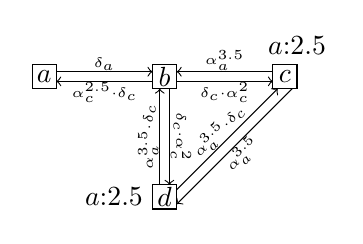
\begin{tikzpicture}[scale=0.87]

  \newcommand\X{50pt}
  \newcommand\Y{-50pt}

  \newcommand\ADD{\alpha}
  \newcommand\DEL{\delta}

  \thickmuskip=0mu
  \medmuskip=0mu
  \thinmuskip=0mu

  \draw[->] (-\X + 5pt, 0 + 2pt ) --
  node[above=-0.3em,font=\tiny]{$\bm{\DEL_{a}}$}
  (0 - 5pt, 0 + 2pt); %% a - b
  \draw[<-] (-\X + 5pt, 0 - 2pt ) --
  node[below=-0.3em,font=\tiny]{$\ADD_{c}^{2.5}\cdot\DEL_{c}$}
  (0 - 5pt, 0 - 2pt); %% b - a 

  \draw[<-] (0 +5pt, 0 + 2pt) --
  node[above=-0.3em, font=\tiny]{$\ADD_a^{3.5}$}
  (\X -5pt, 0 + 2pt); %% c - b
  \draw[->] (0 +5pt, 0 - 2pt) --
  node[below=-0.3em, font=\tiny]{$\DEL_{c}\cdot\ADD_c^{2}$}
  (\X -5pt, 0 - 2pt); %% b - c

  \draw[->] (0 + 2pt, 0 - 5pt) --
  node[above=-0.3em, font=\tiny, sloped]{$\DEL_{c}\cdot\ADD_c^{2}$}
  (0 + 2pt, \Y + 5pt); %% b - d
  \draw[->] (0 - 2pt, \Y + 5pt) --
  node[above=-0.3em, font=\tiny, sloped]{$\ADD_{a}^{3.5}\cdot\DEL_c$}
  (0 - 2pt, 0 - 5pt);  %% d - b
  
  \draw[<-] (\X - 3pt, 0 - 5pt) --
  node[above=-0.3em, font=\tiny, sloped]{$\ADD_{a}^{3.5}\cdot\DEL_{c}$}
  (0 + 5pt, \Y + 3pt); %% d - c
  \draw[->] (\X + 3pt, 0 - 5pt) --
  node[below=-0.3em, font=\tiny, sloped]{$\ADD_{a}^{3.5}$}
  (0 + 5pt, \Y - 3pt); %% c - d



  
  \draw[fill=white] (-\X, 0) node{$\bm{a}$} +(-5pt, -5pt) rectangle +(5pt, 5pt);  
  \draw[fill=white] (0, 0) node{$\bm{b}$} +(-5pt, -5pt) rectangle +(5pt, 5pt);
  \draw[fill=white] (\X, 0) node{$\bm{c}$} +(-5pt, -5pt) rectangle +(5pt, 5pt);
  \draw[fill=white] (0, \Y) node{$\bm{d}$} +(-5pt, -5pt) rectangle +(5pt, 5pt);
  
  % \draw (-\X+5pt, 5pt) node[above left]{$\DEL_a$};
  \draw (\X+5pt, 5pt) node[above]{$\bm{a: 2.5}$}; %% c
  % \draw (0, 5pt) node[above]{$\bm{a: 1.5}$}; %% b
  \draw (-5pt, \Y) node[left]{$\bm{a: 2.5}$}; %% d


\end{tikzpicture}
}
    \hspace{5pt}
    \subfloat[Part D][\label{fig:delD}Processes discard remaining messages.
      Process $b$ does not deliver $\delta_a$, for it already removed $a$ when
      Partition $c$ dominated it. Processes $c$ and $d$ remain in an incorrect
      partition.]{
\begin{tikzpicture}[scale=0.87]

  \newcommand\X{50pt}
  \newcommand\Y{-50pt}

  \newcommand\ADD{\alpha}
  \newcommand\DEL{\delta}

  \thickmuskip=0mu
  \medmuskip=0mu
  \thinmuskip=0mu

  \draw[->] (-\X + 5pt, 0 + 2pt ) --
  node[above=-0.3em,font=\tiny]{$\DEL{c}\cdot\ADD_c^{4}\cdot$\textcolor{\WRONG}{$\bm{\DEL_{a}}$}}
  (0 - 5pt, 0 + 2pt); %% a - b
  \draw[<-] (-\X + 5pt, 0 - 2pt ) --
  (0 - 5pt, 0 - 2pt); %% b - a 

  \draw[<-] (0 +5pt, 0 + 2pt) --
  (\X -5pt, 0 + 2pt); %% c - b
  \draw[->] (0 +5pt, 0 - 2pt) --
  (\X -5pt, 0 - 2pt); %% b - c

  \draw[->] (0 + 2pt, 0 - 5pt) --
  (0 + 2pt, \Y + 5pt); %% b - d
  \draw[->] (0 - 2pt, \Y + 5pt) --
  (0 - 2pt, 0 - 5pt);  %% d - b
  
  \draw[<-] (\X - 3pt, 0 - 5pt) --
  (0 + 5pt, \Y + 3pt); %% d - c
  \draw[->] (\X + 3pt, 0 - 5pt) --
  (0 + 5pt, \Y - 3pt); %% c - d



  
  \draw[fill=white] (-\X, 0) node{$\bm{a}$} +(-5pt, -5pt) rectangle +(5pt, 5pt);  
  \draw[fill=white] (0, 0)
  node[color=\WRONG]{$\bm{b}$} +(-5pt, -5pt)
  rectangle +(5pt, 5pt);
  \draw[fill=white] (\X, 0) node{$\bm{c}$} +(-5pt, -5pt) rectangle +(5pt, 5pt);
  \draw[fill=white] (0, \Y) node{$\bm{d}$} +(-5pt, -5pt) rectangle +(5pt, 5pt);
  
  % \draw (-\X+5pt, 5pt) node[above left]{$\DEL_a$};
  \draw (\X+5pt, 5pt) node[above, color=\WRONG]{$\bm{a: 2.5}$}; %% c
  % \draw (0, 5pt) node[above]{$\bm{a: 1.5}$}; %% b
  \draw (-5pt, \Y) node[left, color=\WRONG]{$\bm{a: 2.5}$}; %% d


\end{tikzpicture}
}
  \end{center}
  \caption{\label{fig:del}Partition removals cannot rely only on
    current partition, for it may lead to either inconsistent
    partitioning, or every process receiving every broadcast.}
\end{figure*}

%%% Local Variables: 
%%% mode: latex
%%% TeX-master: "../paper"
%%% ispell-local-dictionary: "english"
%%% End: 

